\documentclass [a4paper,12pt,titlepage]{article}
\usepackage[utf8]{inputenc}
\usepackage[french]{babel}
\setcounter{section}{+1} % Change the number representing sections

% Outils page de garde
\usepackage{tikz}
\usepackage{circuitikz}
\usepackage{pgffor}
\usepackage{fancyhdr}

\usepackage[a4paper,top=2cm,bottom=2cm,left=1.5cm,right=1.5cm,marginparwidth=1.75cm]{geometry}
\usepackage{hyperref}
\usepackage{multirow}
\usepackage{color}
\usepackage{enumitem}
\usepackage{amsmath}
\usepackage{mathtools}
\usepackage{amssymb}
\usepackage{graphicx}
\usepackage{float}
\usepackage{physics}
\usepackage{xcolor}
\usepackage{sistyle}
\usepackage{textcomp}
\usepackage{gensymb}
\usepackage{lastpage}
\usepackage{caption}
\usepackage{subcaption}
\usepackage{multicol}
% \usepackage[margin=1in]{geometry}
\usepackage[parfill]{parskip}
\usepackage[overload]{empheq}
\usepackage{amsfonts}
\usepackage{amssymb}
\usepackage{amsmath}
\usepackage{verbatim} % Introduire des commentaires
\usepackage{xcolor}
\usepackage{graphicx}
\usepackage{hyperref}
\usepackage{caption}
\usepackage{subcaption}
\usepackage{enumitem}

% euro symbol
\usepackage[gen]{eurosym}

% \usepackage{diffcoeff} % Permet d'écrire facilement les dérivées.

\usepackage{float}
\usepackage{graphicx}

\newcommand\tab[1][1cm]{\hspace*{#1}}
\setlength{\parindent}{0pt}

\hypersetup{
    colorlinks=true,
    linkcolor=[RGB]{0,35 ,173},
    filecolor=black,      
    urlcolor=cyan,
}

\pagestyle{fancy}
\fancyhead[L]{Bouhy Maxime / Hogge Louis / Kaiser François / Louveau Simon }
\fancyhead[C]{}
\fancyhead[R]{Supply Chain Management}
\fancyfoot[c]{Page : \thepage/\pageref{LastPage}}
\renewcommand{\footrulewidth}{0.4pt}
\def\changemargin#1#2{\list{}{\rightmargin#2\leftmargin#1}\item[]}
\let\endchangemargin=\endlist 

\begin{document}
%%%%%%%%%%%%%%%%%%%%%%%%%%%%%%%%%%%%%%%%%%%%%%%%%%%%%%%%%%%%%%%%%%%%%%%%%%%%%%%%%%%%%%%%%

\begin{titlepage}
\begin{tikzpicture}[remember picture,overlay]
  \coordinate [above=0cm] 
  (bottompoint) at (current page.south);
\node[anchor=base, minimum width=\paperwidth] (footernator) at (bottompoint){
    
\includegraphics[width=\paperwidth, height=\paperheight]{Gray Minimalist Annual Report Cover Page.png}
    };
\end{tikzpicture}
\end{titlepage}
\newpage
\tableofcontents

%%%%%%%%%%%%%%%%%%%%%%%%%%%%%%%%%%%%%%
\newpage
\section*{Introduction}
\addcontentsline{toc}{section}{Introduction}
This report was done in order to propose a new strategy for production and distribution planning at Marinero that maximizes its profit that is the difference between total revenue and total cost. It is separated into two sections (Mathematical Model and Obtained Results). Results and analysis are presented in the second section.

%%%%%%%%%%%%%%%%%%%%%%%%%%%%%%%%%%%%%%
\section*{Mathematical Model}
\addcontentsline{toc}{section}{Mathematical Model}
\subsection{Sets}
\begin{enumerate}
    \item[-] Set of products N = \{1, 2, 3, 4, 5\}
    \item[-] Set of production plants P = \{1, 2, 3\}
    \item[-] Set of sales centers S = \{1 (Fiumicino), 2 (Genova), 3 (Rimini), 4 (Bari), 5(Cagliari), 6 (Palermo), 7 (Milano), 8 (Salerno)\}
    \item[-] Set of markets M = \{firm, individual\}
    \item[-] Set of months, periods K = \{1, 2, 3, 4, 5, 6\}
\end{enumerate}
\subsection{Parameters}
\begin{enumerate}
    \item[-] TransportCost($P_{i}$, $S_{i}$)
    \item[-] InventoryCost($S_{i}$, $N_{i}$)
    \item[-] ProductVolume($N_{i}$)
    \item[-] UpperLimitManHour($P_{i}$)
    \item[-] LowerLimitManHour($P_{i}$)
    \item[-] ManMonthCost($P_{i}$)
    \item[-] ManHourAvail($P_{i}$)
    \item[-] ManHourUsage($P_{i}$, $N_{i}$)
    \item[-] OpeningPlantCost($P_{i}$)
    \item[-] OpeningCenterCost($S_{i}$)
    \item[-] DemandMarket($K_{i}$, $N_{i}$)
    \item[-] Prices($N_{i}$, $M_{i}$)
    \item[-] PercentageDemandMarket($P_{i}$, $M_{i}$)
\end{enumerate}
\subsection{Decision Variables}
\begin{enumerate}
    \item[-] QuantityShipped($K_{i}$, $P_{i}$, $S_{i}$, $N_{i}$)
    \item[-] Workers($K_{i}$, $P_{i}$)
    \item[-] SalesCenterOpen($S_{i}$)
    \item[-] PlantsOpen($P_{i}$)
    \item[-] ProductSales($K_{i}$, $S_{i}$, $N_{i}$, $M_{i}$)
    \item[-] QuantityStored($K_{i}$, $S_{i}$, $N_{i}$)
\end{enumerate}

\newpage
\subsection{Constraints}
\begin{enumerate}
    \item[-] InventoryBalanceM1($K_{i}, S_{i}, N_{i}$) :
    \begin{equation*}
    \begin{split}
    \hspace*{-5cm}
    QuantityStored(K_{i}, S_{i}, N_{i}) &= \sum_{P_{i}}QuantityShipped(K_{i}, P_{i}, S_{i}, N_{i}) \\
    &- \sum_{M_{i}}ProductSales(K_{i}, S_{i}, N_{i}, M_{i})
    \end{split}
    \end{equation*}
    \item[-] InventoryBalanceOtherM($K_{i}, S_{i}, N_{i}$) :
    \begin{equation*}
    \begin{split}
    \hspace*{-5cm}
    QuantityStored(K_{i}, S_{i}, N_{i}) & = QuantityStored(K_{i-1}, S_{i}, N_{i}) \\ & + \sum_{P_{i}}QuantityShipped(K_{i}, P_{i}, S_{i}, N_{i}) \\
    & - \sum_{M_{i}}ProductSales(K_{i}, S_{i}, N_{i}, M_{i})
    \end{split}
    \end{equation*}
    \item[-] DemandSatisfaction($K_{i}, N_{i}, M_{i}$) :
    \begin{equation*}
    \begin{split}
    \hspace*{-4.5cm}
    \sum_{S_{i}}ProductSales(K_{i}, S_{i}, N_{i}, M_{i}) &\leq DemandMarket(K_{i}, N_{i}) \; \times \\ & PercentageDemandMarket(P_{i}, M_{i})
    \end{split}
    \end{equation*}
    \item[-] ProductionCapacity($K_{i}$, $P_{i}$) :
    \begin{equation*}
    \begin{split}
    \hspace*{-4.3cm}
    \sum_{N_{i}}ManHourUsage(P_{i}, N_{i}) \; \times & \sum_{S_{i}}QuantityShipped(K_{i}, P_{i}, S_{i}, N_{i}) \leq \\ & Workers(K_{i},P_{i}) \times ManHourAvail(P_{i})
    \end{split}
    \end{equation*}
    \item[-] SalesCenterLimit :
    \begin{equation*}
    \begin{split}
    \hspace*{-8.35cm}
    \sum_{S_{i}}SalesCenterOpen(S_{i}) \leq 7
    \end{split}
    \end{equation*}
    \item[-] PlantsOpening($P_{i}$) :
    \begin{equation*}
    \begin{split}
    \hspace*{-2.5cm}
    \sum_{K_{i}}\sum_{S_{i}}\sum_{N_{i}} QuantityShipped(K_{i}, P_{i}, S_{i}, N_{i}) \leq PlantsOpen(P_{i}) \; \times 10000000000
    \end{split}
    \end{equation*}
    \item[-] SalesCenterOpening($S_{i}$) :
    \begin{equation*}
    \begin{split}
    \hspace*{-1cm}
    \sum_{K_{i}}\sum_{N_{i}}\sum_{M_{i}} ProductSales(K_{i}, S_{i}, N_{i}, M_{i}) \leq SalesCenterOpen(S_{i}) \; \times 100000000000000
    \end{split}
    \end{equation*}
    \item[-] WorkersUpperBounds($K_{i}$, $P_{i}$) :
    \begin{equation*}
    \begin{split}
    \hspace*{-0.69cm}
    Workers(K_{i},P_{i}) \leq UpperLimitManHour(P_{i}) \; \times PlantsOpen(P_{i})
    \end{split}
    \end{equation*}
    \item[-] WorkersLowerBounds($K_{i}$, $P_{i}$) :
    \begin{equation*}
    \begin{split}
    \hspace*{-0.69cm}
    Workers(K_{i},P_{i}) \leq LowerLimitManHour(P_{i}) \; \times PlantsOpen(P_{i})
    \end{split}
    \end{equation*}
\end{enumerate}

\newpage
\subsection{Objective Function}
MaxProfit $\rightarrow$ Maximise TotalProfit
\begin{enumerate}
    \item[-] TotalProfit = Revenue - Cost
    \item[-] Revenue = $\sum_{K_{i}}\sum_{S_{i}}\sum_{N_{i}}\sum_{M_{i}}(ProductSales(K_{i}, S_{i}, N_{i}, M_{i}) \; \times Prices(N_{i}, M_{i}))$
    \item[-] Costs = ActivationCosts + TransportationCosts + InventoryHoldingCosts + LaborCosts
    \item[-] ActivationCosts =
    \begin{equation*}
    \begin{split}
    & \; \; \; \; \sum_{P_{i}} (PlantsOpen(P_{i}) \; \times OpeningPlantCost(P_{i}) \; \times 1000) \\ & + \sum_{S_{i}}(SalesCenterOpen(S_{i}) \; \times OpeningCenterCost(S_{i}) \; \times 1000)
    \end{split}
    \end{equation*}
    \item[-] TransportationCosts =
    \begin{equation*}
    \begin{split}
    \hspace*{-0.3cm}
    \sum_{K_{i}}\sum_{P_{i}}\sum_{S_{i}}\sum_{N_{i}} (QuantityShipped(K_{i}, P_{i}, S_{i}, N_{i}) \; \times ProductVolume(P_{i}) \; \times TransportCost(P_{i}, S_{i}))
    \end{split}
    \end{equation*}
    \item[-] InventoryHoldingCosts =
    \begin{equation*}
    \begin{split}
    \hspace*{-5.3cm}
    \sum_{K_{i}}\sum_{S_{i}}\sum_{N_{i}}(QuantityStored(K_{i}, S_{i}, N_{i}) \; \times InventoryCost(S_{i}, N_{i}))
    \end{split}
    \end{equation*}
    \item[-] LaborCosts =
    \begin{equation*}
    \begin{split}
    \hspace*{-8cm}
    \sum_{K_{i}}\sum_{P_{i}}(Workers(K_{i}, P_{i}) \; \times ManMonthCost(P_{i}))
    \end{split}
    \end{equation*}
\end{enumerate}

\newpage

\section*{Obtained Results}
\addcontentsline{toc}{section}{Obtained Results}

% You are asked to propose a new strategy for production and distribution planning at Marinero that maximizes its profit that is the difference between total revenue and total cost.
% • The total cost will include:
% – the activation costs of the facilities,
% – production and distribution costs, 
% – inventory holding costs,
% – labor costs.

The following is Marinero's ideal production and distribution planning strategy, as determined by the AIMMS analysis:

\begin{enumerate}
    \item[-] \textbf{Activation costs of the plants:}
    
    To reduce activation costs, the strategy focuses on giving production priority at the facilities that are the most economical. The analysis suggests that the \textit{Cagliari} and \textit{Cosenza} facility should serve as the major production site.

    \item[-] \textbf{Production and distribution costs:}

    The strategy proposes focusing on items with higher demand and profit margins in order to reduce production and distribution costs. In terms of distribution, the plan advises utilizing \textit{Cagliari} as the primary sales hub and \textit{Bari} and \textit{Salerno} as the secondary sales hubs.

    \item[-] \textbf{Inventory holding costs:}

    By coordinating production with demand, it is evident from the data analysis that inventory holding costs can be greatly decreased. The plan also suggests reducing inventories for products with low demand.

    \item[-] \textbf{Labor costs:}
    
    The approach recommends employing the maximal workforce at each production plant each month.
\end{enumerate}

With revenue of \euro{14,761,211.33} and total cost of \euro{2,012,204.014}, we managed to make a total profit of \euro{12,749,007.32}.

In conclusion, Marinero's ideal approach to production and distribution planning prioritizes the \textit{Cagliari} facility, focuses on high-demand products, synchronizes production with demand to reduce inventory holding costs, and makes effective use of the personnel. By putting this plan into action, Marinero will be able to increase its profit by decreasing overall costs and raising total revenue.

\newpage

\begin{figure}[H]
  \centering
  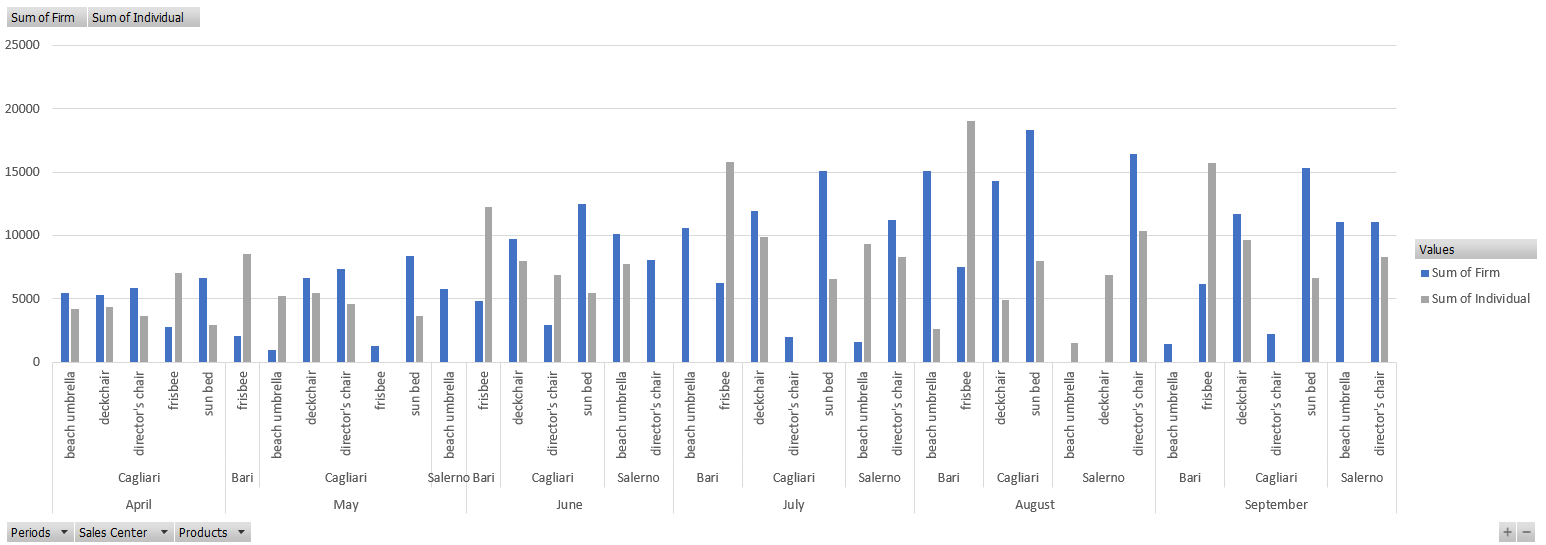
\includegraphics[width=1\textwidth]{graph1.png}
  \caption{Monthly sales of each product according to the sales centers and target market }
  \label{fig: graph1}
\end{figure}

\begin{figure}[H]
  \centering
  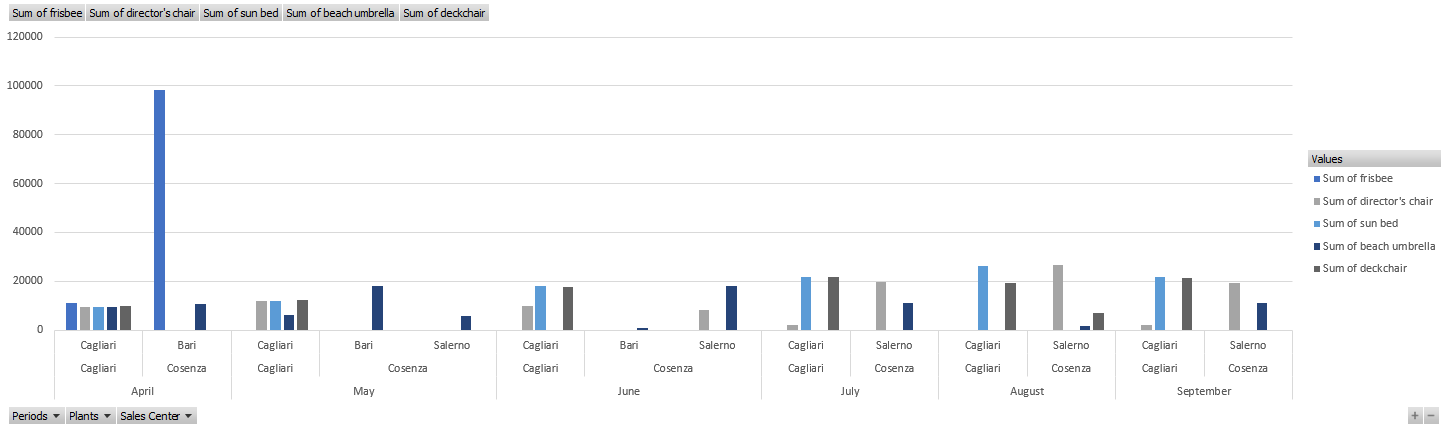
\includegraphics[width=1\textwidth]{graph2.png}
  \caption{Monthly export of each product from a production plant to the corresponding sales center}
  \label{fig: graph2}
\end{figure}

\begin{figure}[H]
    \begin{minipage}[b]{0.5\linewidth}
        \centering 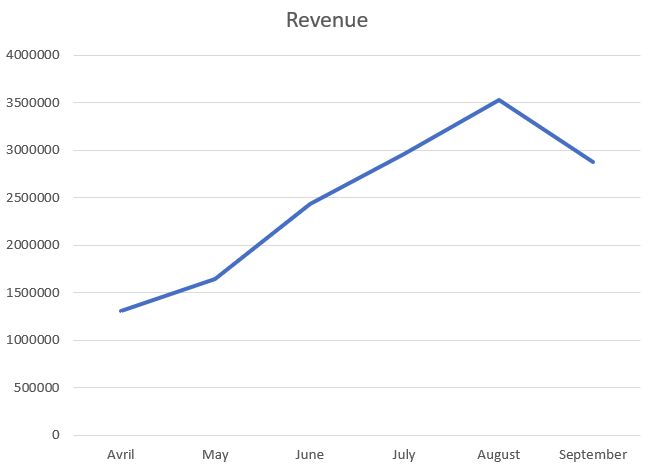
\includegraphics[scale=0.3]{graph3.png}
        \caption{Monthly Revenue}
    \end{minipage}\hfill
    \begin{minipage}[b]{0.5\linewidth}
        \centering 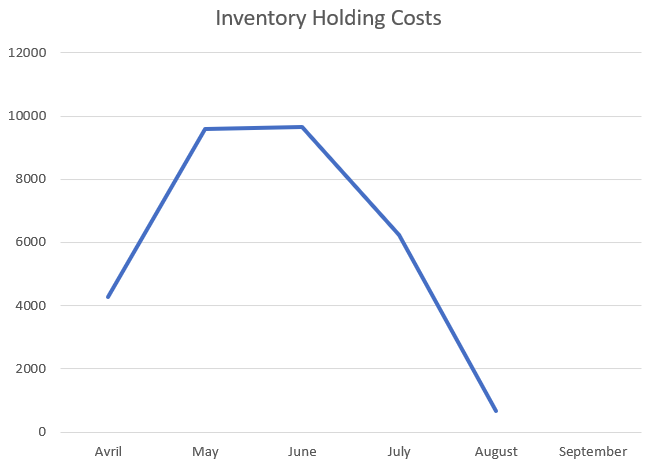
\includegraphics[scale=0.3]{graph4.png}
        \caption{Monthly inventory holding costs}
    \end{minipage}
\end{figure}

\end{document}
